%
%%%%%%%%%%%%%%%%%%%%%%%%%%%%%%%%%%%%%%%%%%%%%%%%%%%%%%%%%%
%
%  A N F O R D E R U N G E N   &   K O N Z E P T Z I O N
%
%%%%%%%%%%%%%%%%%%%%%%%%%%%%%%%%%%%%%%%%%%%%%%%%%%%%%%%%%%
\chapter{Anforderungen und Konzeption}
\label{cha:methodik}
%
Unter funktionalen Anforderungen versteht man konkrekte Funktionalitäten, welche die Anwendung leisten soll. Die Anwendung lässt sich in mehrere Module aufteilen, die dem User zu Verfügung stehen. Im Folgenden werden die funktionalen Anforderungen erläutert.
%
%%%%%%%%%%%%%%%%%%%%%%%%%%%%%%%%%%%%%%%%%%%%%%%%%%%
%
% Problemanalyse
%
%%%%%%%%%%%%%%%%%%%%%%%%%%%%%%%%%%%%%%%%%%%%%%%%%%%
%
\section{Funktionale Anforderungen}
\label{sec:problemanalyse}
%
Unter funktionalen Anforderungen versteht man konkrekte Funktionalitäten, welche die Anwendung leisten soll. Die Anwendung lässt sich in mehrere Module aufteilen, die dem User zu Verfügung stehen. In diesem Kaptitel werden sowohl die funktionalen also auch die nicht funktionalen Anforderungen beschrieben. Es handelt sich zwar um ein echtes Projekt, wobei es sich vorerst um eine prototypische Entwicklung handelt. Als Anforderung vom Hersteller gilt nur, dass der Konfigurator einen Bestellvorgang für den Kunden und das Unternehmen vereinfacht. Dabei soll durch innovative Gestaltung und Programmierung des Konfigurators eine performante Lösung entwickelt werden. Das Ergebnis sollte zum bisherigen Webauftritt des Unternehmens passen. Nun wollen wir uns die Anforderungen im Details anschauen. Anschließend wird das Konzept des Webanwendung vorgestellt.

\renewcommand{\arraystretch}{1.8}
\begin{table}[h]
	\begin{tabular}{|r|c|p{8.5cm}|}
		\hline
		\textbf{Nr.} & \textbf{Bezeichnung} & \textbf{Beschreibung} \\
		\hline
		1 & Auswahl des Bechers & Der Benutzer kann zwischen verschiedenen Bechergrößen wählen. \\
		\hline
		2 & Interaktionen & Der Benutzer kann beispielsweise den Becher transformieren oder an den Becher heranzoomen. \\
		\hline
		3 & Upload des Designs & Der Benutzer kann nach sein Design entsprechende der Druckvorgaben hochlade.n \\
		\hline
		4 & Zusatzoptionen & Der Benutzer kann bestimmte Zusatzoptionen auswählen. \\
		\hline
		5 & Übersicht anzeigen & Der Benutzer kann sich eine Übersicht seiner Konfiguration ansehen. \\
		\hline
		6 & Konfiguration speichern & Der Benutzer kann seinen konfigurierten Becher speichern. \\
		\hline
	\end{tabular}
\caption{Übersicht der funktionalen Anforderungen}
\end{table}
%
\paragraph{3D Vorschau des Bechers}
Zunächst ist wichtig, das die 3D Darstellung des Bechers umgesetzt wird. Dabei spielt das Design, welches der User hochladen wird, erst einmal keine Rolle. Schon beim Start wird Standardmäßig des 3D-Modell eines Bechers angezeigt. Von den Mehrwegbechern sind vier verschiedene Größen vorhanden. Dem Benutzer soll es möglich sein über das Konfigurationsmenü eine beliebige Größe auszuwählen. Ohne lange Wartezeiten muss sich das 3D-Modell des Bechers dementsprechend aktualisieren.\\
Falls der User schon ein Design hochgeladen hat und die Größe nun ändern möchte, wird das Design gelöscht und muss erneut hochgeladen werden. Grund dafür sind die unterschiedlichen Designvorgaben für jede Größe. Man soll vor dem Löschvorgang allerdings einen Warnhinweis bekommen, um ungewolltes Löschen zu vermeiden.
%
\paragraph{Interaktionen}
Da es sich um eine 3D Ansicht handelt, sollte man auch interagieren können. Der Becher kann von Benutzer 360 Grad auf der X-Achse und auf der Y-Achse 180 Grad gedreht werden. Auch eine Zoom-Funktion soll implementiert werden. Damit kann der User näher an den Becher heranzoomen. Es sollte jedoch ein maximaler Zoom eingestellt werden, damit die Ansicht realistisch bleibt. Außerdem soll zur einfachereren Bedienung ein Button erstellt werden, der den Becher wieder in seine Ursprungsposition bringt. Diese Interaktionen sollten sowohl mit der Maus als auch mit Touch-Eingabe funktionieren.
%
\paragraph{Upload des Designs}
Normalerweise kann ein Kunde einen Mehrwegbecher über Flyeralarm\footnote{https://www.flyeralarm.com/de/} drucken lassen. Dabei muss man sich an die Design-Vorgaben halten, die im Datenblatt\footnote{siehe Anhang} definiert sind. Diese unterscheiden sich je nach Größe des Bechers, da es sich ja um ein vollflächigen Druck handelt. Um den Benutzer Arbeit zu ersparen, sollte er das Design genau nach den Vorgaben der Druckerei hochladen. Beim Upload wird die Datei auf das korrekte Seitenverhältnis geprüft. Ohne lange Wartezeit wird nun das Design auf den Becher gerendert und der Kunde kann sich das Ergebnis anschauen. Es sollte auch möglich sein das Design mit einem anderen zu ersetzten. Wie schon erwähnt wird das Design bei ändern der Bechergröße entfernt. Als Dateiformat sind ausschließlich \texttt{png}-Dateien zulässig, weil damit Transarenzen dargestellt werden können.
%
\paragraph{Zusatzoptionen wählen}
Hierbei handelt es sich um optionale Zusatzfunktionen die nicht unbedingt im Rahmen des Bachlorprojektes umgesetzt werden. Eine Zusatzoption wäre das ein und ausblenden des Eichstrichs, der bei den Mehrwegbechern mit aufgedruckt wird. Eine weitere Zusatzangabe des Users wäre eine Eingabe der Stückzahl, die bestellt werden soll. Das wäre sinnvoll wenn der Konfigurator in Zukunft in den Bestellvorgang eingabaut werden soll. Andernfalls hätte der Kunde zumindest die Möglichkeit eine Preisvorschau in der Übersicht zu sehen.
%
\paragraph{Übersicht anzeigen}
Wie gerade erwähnt soll es eine Übersicht geben. In Form einer Tabelle soll dem Kunden nun noch einmal seine Auswahl zusammengefasst werden. Er kann dort die ausgewählte Bechergröße, das hochgeladene Design (den Dateinamen), eventuell die Stückzahl, Preisvorschau und so weiter, sehen. Optional kann eine Druck-Funktion implementiert werden, die es dem Benutzer ermöglicht die Übersicht inkulsive einer Abbildung des Bechers mit dem Design zu drucken bzw. in einer \texttt{pdf}-Datei zu speichern.
%
\paragraph{Konfiguration speichern}
Hierbei handelt es sich wieder um eine optionale Funktion, die wahrscheinlich nicht mehr im Rahmen der Bachlorarbeit umgesetzt werden kann. Wenn ein Benutzer einen Becher konfiguriert hat, ist es durchaus denkbar das er zu späteren Zeiten nocheinmal darauf zurückgreifen möchte. Oder er möchte verschiedene Versionen eines Bechers vergleichen. Deshalb wäre es sinnvoll eine Speicher-Funktion zu implementieren, die einfach und schnell den konfigurierten Becher wiederherstellen kann.
%
%%%%%%%%%%%%%%%%%%%%%%%%%%%%%%%%%%%%%%%%%%%%%%%%%%%
%
% Problemanalyse
%
%%%%%%%%%%%%%%%%%%%%%%%%%%%%%%%%%%%%%%%%%%%%%%%%%%%
%
\section{Nicht Funktionale Anforderungen}
\label{sec:problemanalyse}
%
Mit nicht funktionalen Anforderungen sind Funktionalitäten gemeint, welche die Anwendung \textbf{im Hintergrund} leisten soll. Diese sollen die Usablitiy und performance des Konfigurators verbessern und dem Benutzer somit ein innovatives Erlebnis bieten. In der Tabelle sehen sie eine Übersicht der nicht funktionalen Anforderungen.

\renewcommand{\arraystretch}{1.8}
\begin{table}
	\begin{tabular}{|r|c|p{8.5cm}|}
		\hline
		\textbf{Nr.} & \textbf{Bezeichnung} & \textbf{Beschreibung} \\
		\hline
		1 & Uploadfilter & Der Benutzer kann zwischen verschiedenen Bechergrößen wählen. \\
		\hline
		2 & Bedienungshilfen & Der Benutzer kann beispielsweise den Becher transformieren oder an den Becher heranzoomen. \\
		\hline
		3 & Realistische Design-Darstellung & Der Benutzer kann nach sein Design entsprechende der Druckvorgaben hochlade.n \\
		\hline
		4 & Responsive Webdesign & Der Benutzer kann bestimmte Zusatzoptionen auswählen. \\
		\hline
		5 & Benutzerfreundlich & Der Benutzer kann sich eine Übersicht seiner Konfiguration ansehen. \\
		\hline
		6 & Leistungstark & Der Benutzer kann seinen konfigurierten Becher speichern. \\
		\hline
	\end{tabular}
	\caption{Übersicht der funktionalen Anforderungen}
\end{table}
%
\paragraph{Uploadfilter}
Das Design sollte realistisch gerendert werden. Dazu muss das Design wie in den Druckvorgaben hochgeladen werden. Sonst könnte es zu verzehrt aus sehen oder einfach unscharf. Nach dem Upload bekommt der User eine Rückmeldung, ob die Auflösung des Bildes in Ordnung ist. Falls nicht wird das Bild nicht gespeichert bzw. auf den Becher gerendert und der Benutzer soll das Design in der richtigen Auflösung hochladen. Ein ähnliches Vorgehen wird auch bei der Druckerei Fyleralarm bei einem Upload angewendet. Jedoch wird bei dem Konfigurator nur das Seitenverhältnis bzw. die Auflösung geprüft, nicht der Farbmodus oder andere Vorgaben zum Drucken.
%
\paragraph{Bedienungshilfen}
Ähnlich wie beim Upload des Designs soll der Kunde immer wieder Hinweise bekommen was zu tun ist. Beispielweise wie er den Becher drehen kann oder wo er die Größe des Bechers auswählen kann oder wo er die Übersicht seiner Auswahl sehen kann.
%
\paragraph{Realistisches Design-Rendering}
kubisches Problem
Auch was die 3D-Darstellung angeht, sind nicht viele Vorgaben gegeben, was einen weiten Spielraum lässt. Zunächst muss der Becher in die Szene geladen werden können. Anschließend besteht die Herausforderung darin, ein vom Benutzer hochgeladenes Design realistisch auf den Becher zu projizieren. Dabei muss die kubische Form des Bechers und die Upload-Vorgaben der Druckerei berücksichtigt werden. Der Upload-Vorgang muss einfach und verständlich sein, damit der Benutzer weiß wie er sein Design richtig auf den Becher bekommt. Dabei dürfen die Ladezeiten nicht zu lange sein. Die Anwendung muss möglichst performant laufen, unabhängig von der Plattform.
%
\paragraph{Responsive Webdesign}
Es ist wichtig das der Konfigurator auf verschiedenen Displaygrößen verwendet werden kann. Bei mobilen Geräten wird es schwierig die 3D Ansicht und das gesamte Menu zusammen anzuzeigen. Damit die Inhalte groß genug und gut lesbar sein, wird das Menu auf mobilen Gräten also \textit{Off-Canvas-Menu} implementiert. Somit wird zum einen der Becher schön groß dargestellt und zum anderen werden Menu-Items groß und gut lesbar sein. Der Benutzer eines Smartphones sollte nach Möglichkeit den gleichen Funktionsumfang genießen wie ein Benutzer auf Desktop Geräten. Dabei sollte möglichst innovativ gestalet werden.
%
\paragraph{Benutzerfreundlichkeit}
Die Webanwendung soll benutzerfreundlich sein. Dazu tragen die schon erwähnten Bedienungshilfen bei. Wichtig ist, das der Benutzer immer weiß was der nächste Schritt ist. Um dies zu erreichen ist eine einfache und übersichtliche Gestaltung ist nötig. Sie sollte auf das wesentliche beschränkt sein und nicht überladen wirken.
%
\paragraph{Performant}
Wie die Studie im Kapitel Performance gezeigt hat, mögen Benutzer keine langen Wartezeiten. Bei dem 3D-Konfigurator soll das Laden der 3D Modelle nicht länger als 2ms dauern. Das rendern des Designs auf den Becher ebenfalls nicht länger als 2ms. Die Länge des Uploads vom Design hängt von der Internetverbindung ab, sollte allerdings auch schnell abgeschlossen sein. Das Transfomieren des Models in der 3D szene sollte flüssig funktionieren und keine Verzögerungen enthalten. Alles in allem sollte die gesamte Anwendung performant laufen und im Bezug auf die Leistung an eine Desktopanwendung erinnern. Besonders interessant wird dieser Aspket auf mobilen Geräten, denn auch dort sollte die Anwendung möglichst stabil laufen.
%
%
%%%%%%%%%%%%%%%%%%%%%%%%%%%%%%%%%%%%%%%%%%%%%%%%%%%
%
% Konzept
%
%%%%%%%%%%%%%%%%%%%%%%%%%%%%%%%%%%%%%%%%%%%%%%%%%%%
%
\section{Konzeption}
\label{sec:konzept}
%
Bevor es an die Umsetzung und Implementierung geht, beschäftigt sich dieses Kapitel damit, \textbf{wie} der Konfigurator umgesetzt wird. Um den technischen Aufbau zu verstehen, wird ein Flussdiagramm sowie ein Komponentendiagramm verwendet und im Laufe diesen Kapitels erläutert. Anschließend wird auch der grobe Aufbau der Benutzeroberfläche beschrieben.
\begin{figure}[h]
	\centering
	{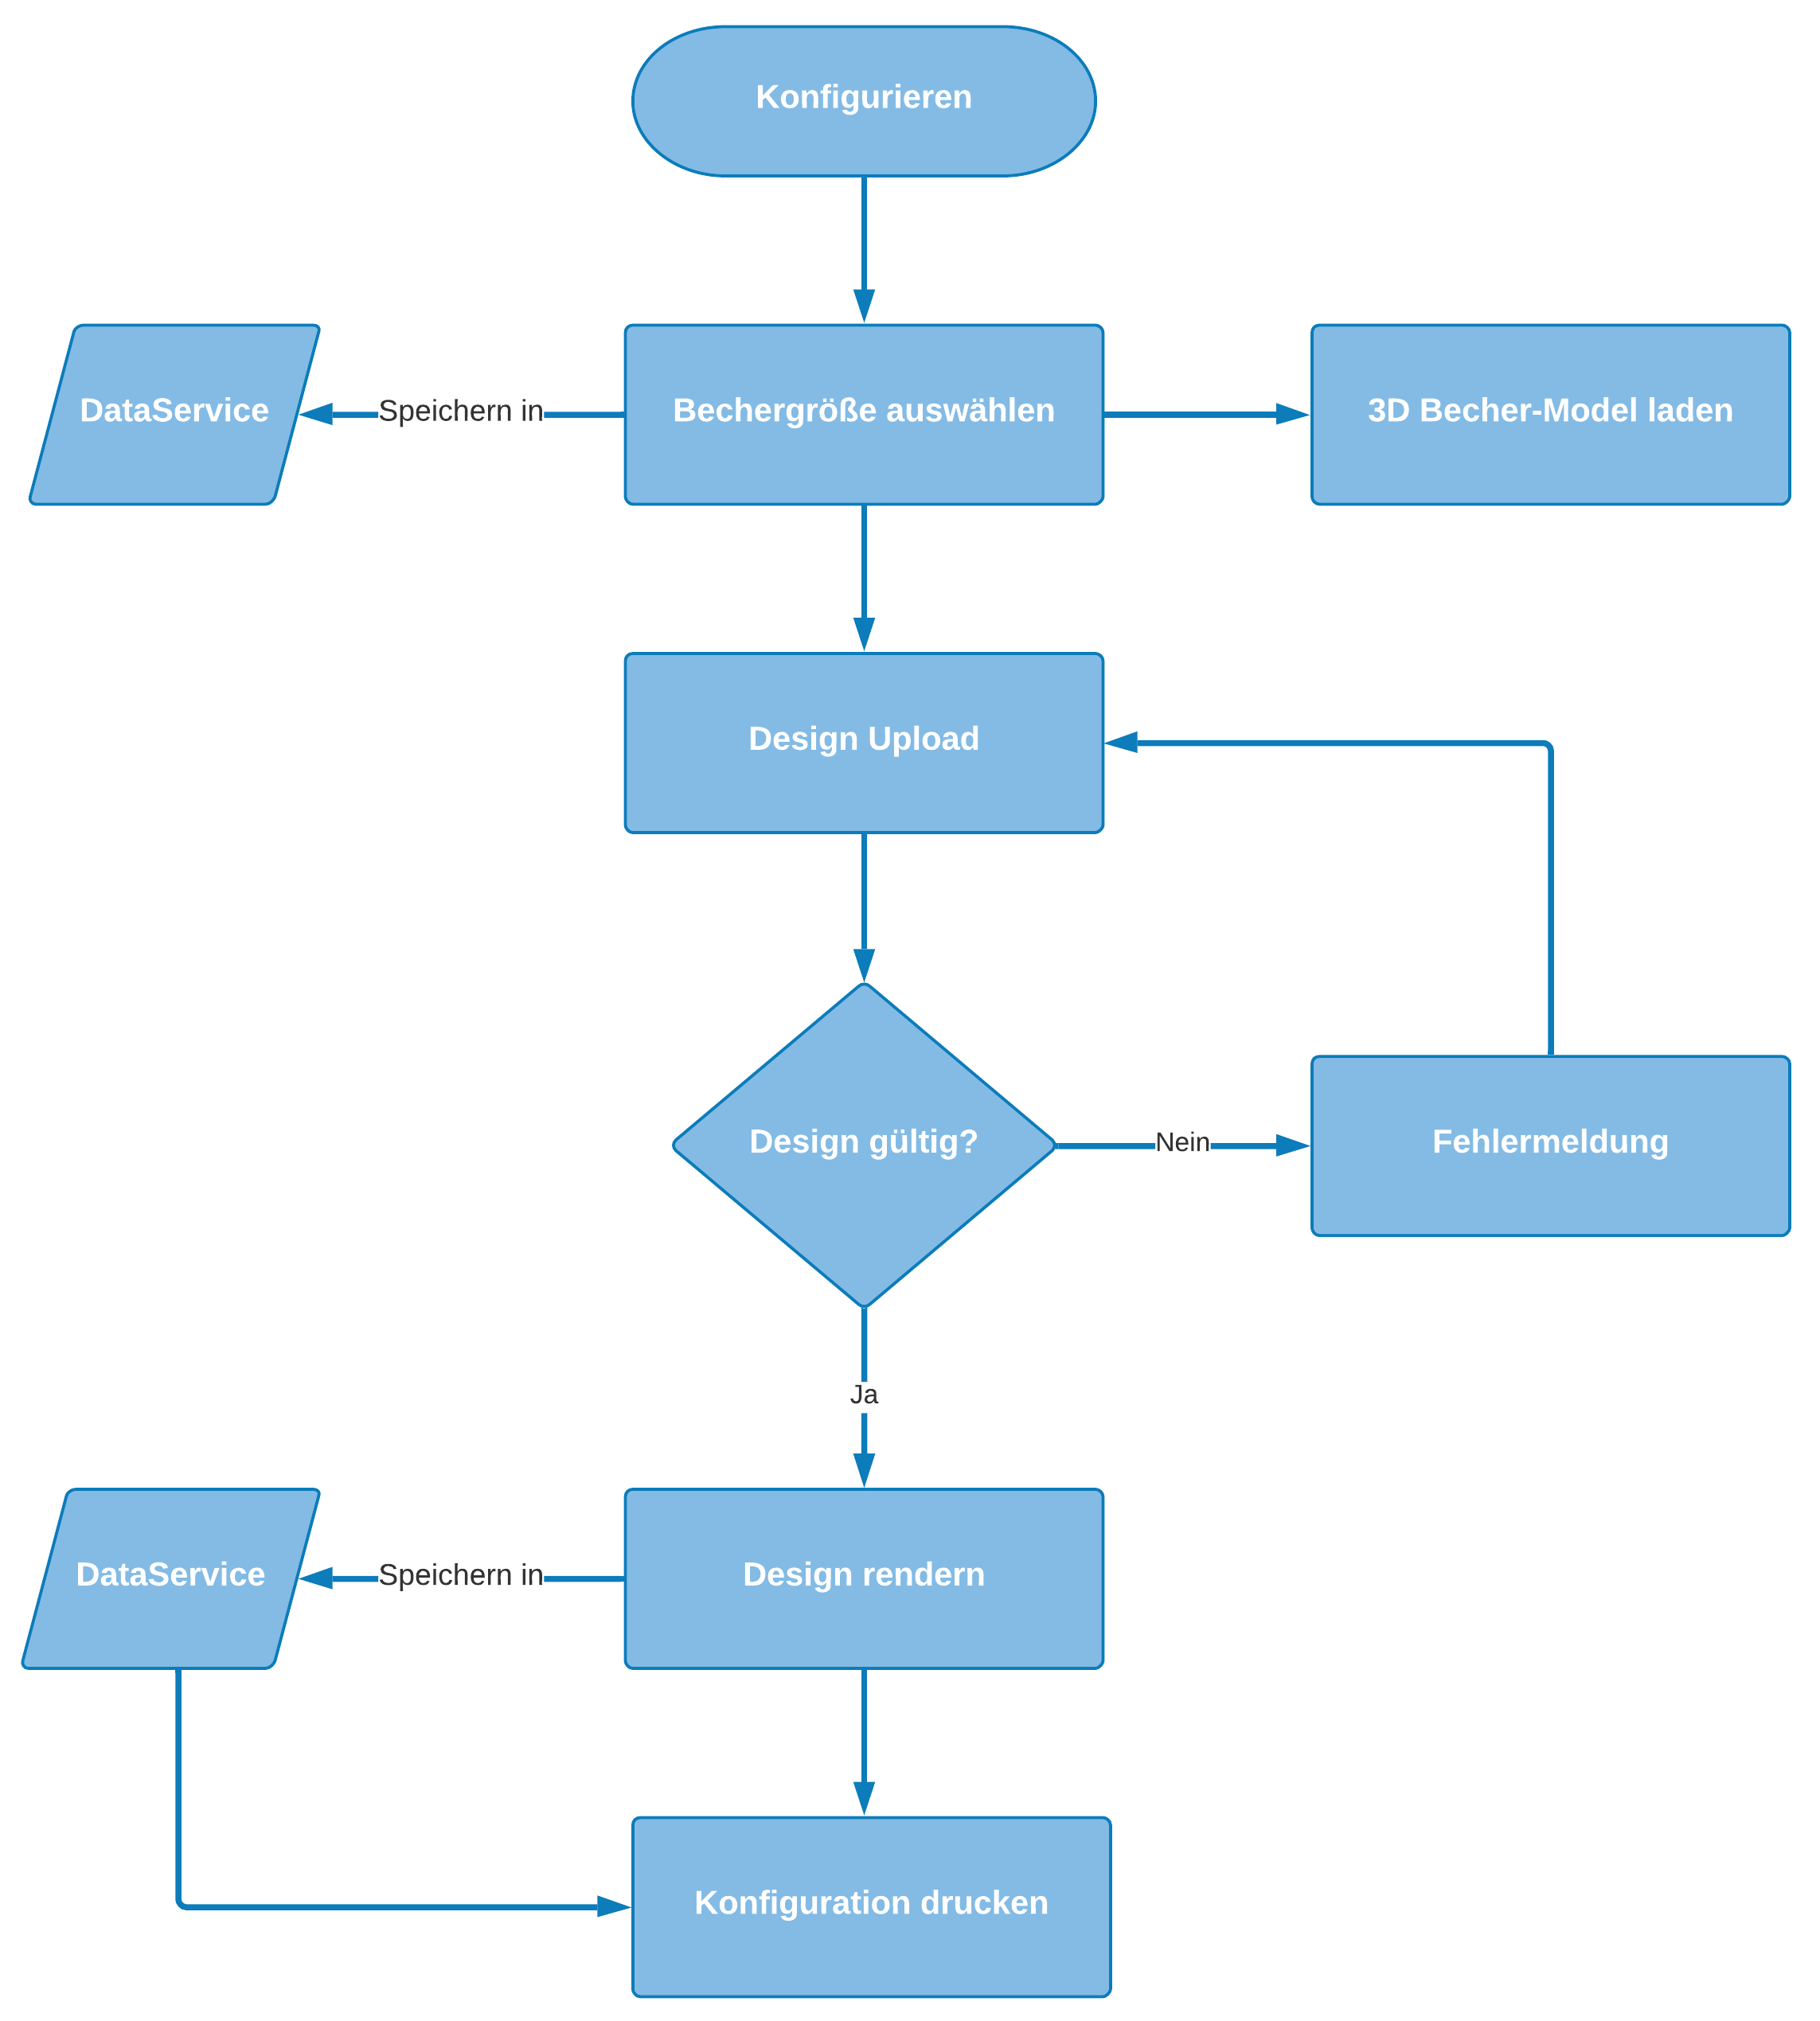
\epsfig{file = methodik/images/flowchart.png, width=9.0cm}}
	\caption[Komponentendiagramm]{\textit{Flussdiagramm der Angular-Anwendung}}
	\label{fig:flowchart}
\end{figure}
 Nachdem alle Funktionen und Vorgaben bekannt sind, sollte man sich über den technischen Ablauf Gedanken manchen. Das Flussdiagramm\footnote{engl. Flowchart sollte hier als Fussnote kurz erkärt werden damit jeder weiß, was genau damit gemeint ist.} in Abbildung \ref{fig:flowchart} zeigt, was während dem Konfigurieren des Bechers geschieht.\\
 Der Konfigurator für Mehrwegbecher beeinhaltet vier verschiedene Größen von Bechern. Als erstes soll der Benutzer eine Bechergröße auswählen. Standardmäßig ist der Becher mit 0,2 Liter als 3D-Model geladen. Falls der Benutzer eine andere Größe wählt, aktualisiert sich das 3D-Model dementsprechend. Anschließend kann der Upload des Becher-Designs erfolgen. Hierbei muss sich der Benutzer an die Druckvorgaben halten. Wenn das Design beispielsweise in einem falsches Dateiformat ist oder eine falsche Auflösung hat, kann das Design nicht hochgeladen werden. Falls alles richtig ist, wird das Design direkt auf den Becher gerendert. Die Wahl der Größe und die hochgeladene Datei werden in dem DataService gespeichert. Am Ende der Konfiguration kann sich der User in der Übersicht alles noch einmal ansehen und bei Bedarf ausdrucken. Dabei werden die Daten aus dem DataService verwendet.  
 
 Jetzt, wo das Flussdiagramm den Ablauf einer Konfiguration beschrieben hat, sollte man sich den Komponenten der Anwendung widmen. Das Komponentendiagramm (siehe Abbildung \ref{fig:ngKomponent}) zeigt die Hauptkomponenten, welche später auch als Angular-Bausteine angelegt werden. Natürlich gibt es noch weitere Kindskomponenten, die in den Hauptkomponenten verwendet werden. Darauf gehen wir aber erst in der Implementierung ein.
\begin{figure}[h]
	\centering
	{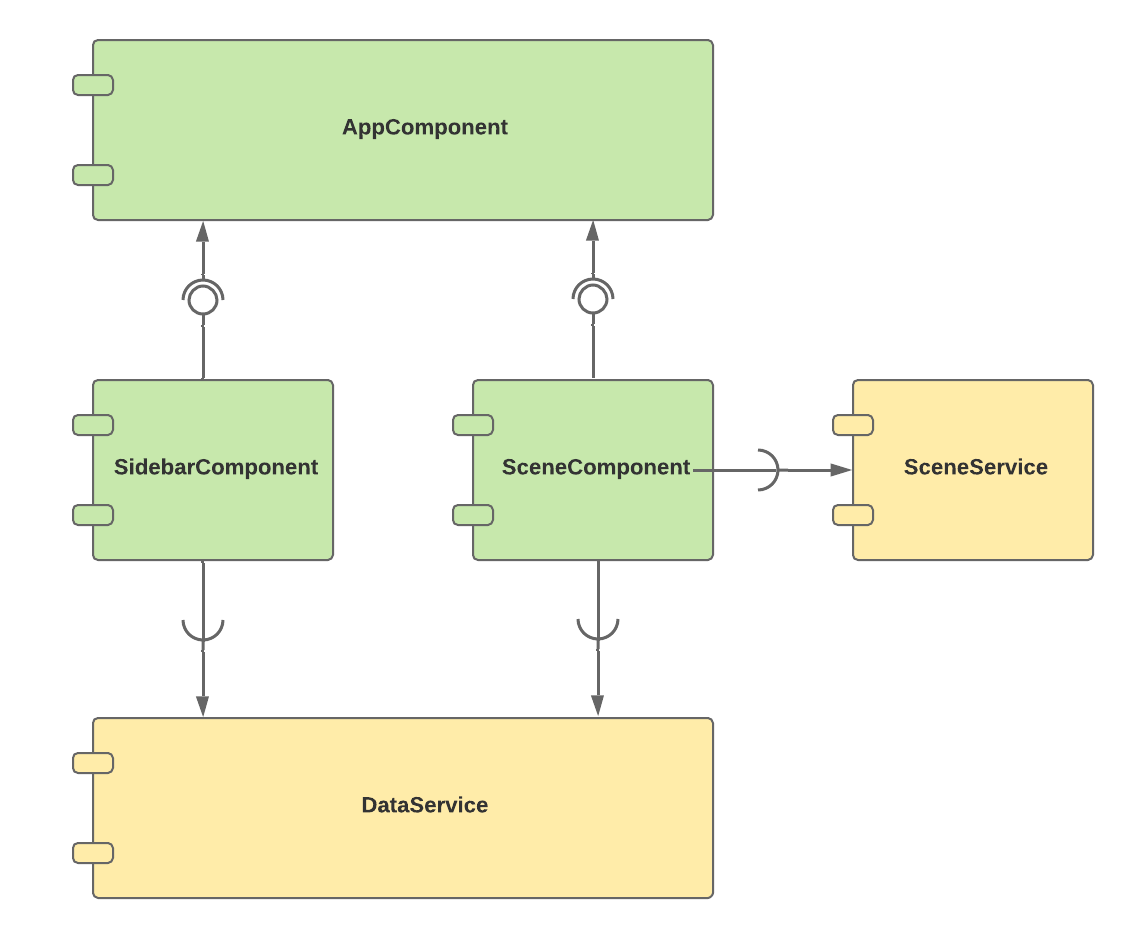
\epsfig{file = methodik/images/komponentnendiagramm.png, width=11.0cm}}
	\caption[Komponentendiagramm]{\textit{Komponentendiagramm der Angular-Anwendung}}
	\label{fig:ngKomponent}
\end{figure} 
Wie wir wissen ist die AppComponent unsere Basis-Komponente, von der alles startet. Nun hat unser Konfigurator eine SidebarComponent, welche das Knofigurationsmenü sowie die Übersicht der Konfigurationen Beeinhaltet. Das Herzstück unserer Angular-Anwendung ist die SceneComponent. Sie zeigt uns den Becher in 3D mit dem hochgeladenen Design. Um eine 3D Szene aufzubauen wird der SceneService verwendet, welcher die 3D Bibliothek Three.js nutzt. Wie schon in dem Flussdiagramm erwähnt befinden sich alle Konfigurations-Daten in dem DataService, welcher global für alle Komponenten bzw. Module zugänglich ist. Damit sollte der technische Aufbau der Anwendung klar sein.

Beschäftigen wir uns nun mit der grafischen Benutzeroberfläche (UI). Am Anfang war ein 3-Schritte-Konfigurator geplant. Der Benutzer sollte also in drei Schritten seinen Becher konfigurieren. Da der Konfigurator nur wenige Einstellmöglichkeiten hat, ist es am benutzerfreundlichsten alles auf einer Seite zu konfigurieren. Somit ist die Webanwendung sehr einfach gehalten und so aufgebaut, dass eine mobile Anpassung leicht umzusetzen ist. Wie in der Abbildung zu sehen ist auf der linken Seite die 3D Szene mit WebGL aufgebaut. Hier kann der User seinen Becher betrachten oder ihn auch transformieren. Auf der rechten Seite befindet sich die Sidebar. Darin ist die komplette Menüführung mit den Konfigurationseinstellungen vorhanden, sowie die Übersicht aller gewählten Einstellungen. Das Menü ist hierarchisch aufgebaut, sodass der Benutzer erst die Größe des Bechers auswählt. Anschließend kann er sein Design hochladen und danach noch optionale Einstellungen wählen. Innerhalb der Sidebar befindet sich auch die Übersicht in Form einer Tabelle. Bei Tablets befindet sich die Sidebar unterhalb der 3D Ansicht. Auf Smartphones ist die Sidebar als Off-Canvas-Menu gelöst. Somit ist das Menü dann vollflächig (siehe Abbildung).
\begin{figure}[h]
	\centering
	{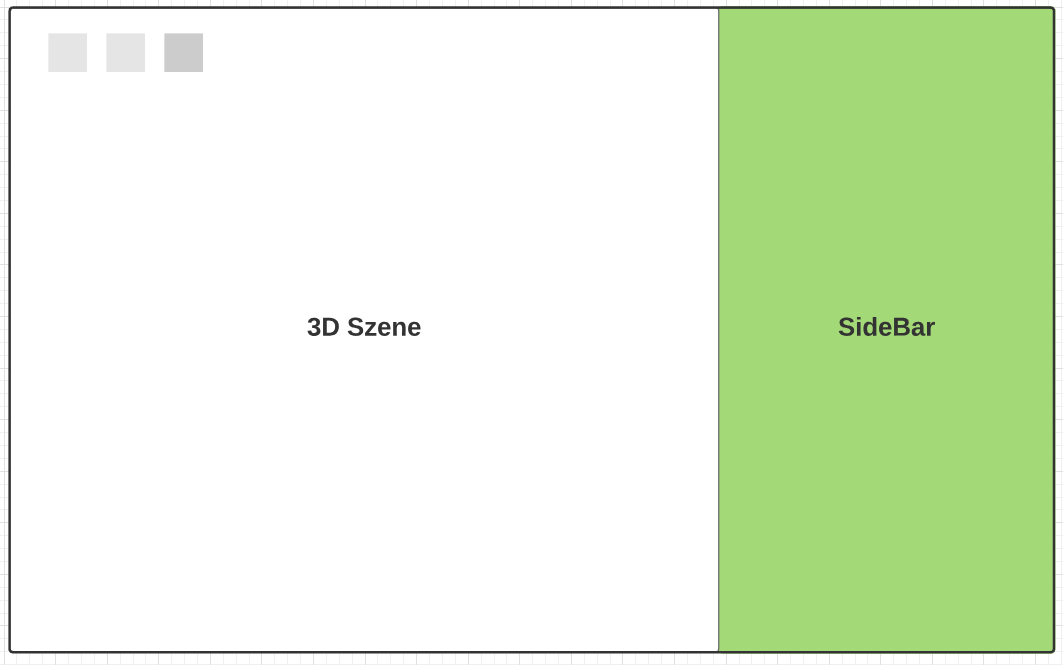
\epsfig{file = methodik/images/mockup.png, width=11.0cm}}
	\caption[Mockup]{\textit{Mockup der Angular-Anwendung}}
	\label{fig:mockup}
\end{figure}

\paragraph{Styles}Der Schwerpunkt des Bachlorprojektes liegt bei der Entwicklung mit Angular und mit WebGL. Deshalb soll nicht viel Zeit für das Styling verwendet werden. Trotzdem soll es ein gutes und innovatives Design geben. Als Grundlage werden die Styles der Unternehmenswebseite sowie Bootstrap verwendet. Somit sind grundlegende Styles wie Schrift und Farben schon festgelegt und müssen nicht mehr betrachtet werden.



• Konzept (UML und weitere Diagramme)
• Mokups der Einzelnen Screens
• Responsive Layout Ideen \\
%